%!TEX root = ../BGP_for_networks_who_peer.tex
\chapter{Traffic Engineering}
\label{ch:trafficengineering}
About half an hour after deploying BGP on your router and setting up eBGP sessions to your upstreams (I assume you have more than one) and peers (peering makes sense, remember?) you will be unhappy with the default decisions BGP makes on where to send your traffic. Half an hour is an optimistic estimation.

So you want to influence BGP. Everybody does. This chapter should give you a toolset to do this. It is up to you to decide which of these tools are useful for you. All networks are different. All use cases are different. Sometimes you need a sledgehammer; sometimes you need tweezers.

As a lot of the things explained here are a matter of personal opinion, the tone of this chapter might be a little ``lighter'' than the rest of this book. Nevertheless it will stick to the facts and give you a toolset you can use.

\section{Remarks about wording}
``\emph{Peer}'' in this chapter will be used as a synonym for a peering partner, an upstream provider, or a BGP customer; so, someone you exchange prefixes with via eBGP.

\section{Tools for outgoing traffic - received prefixes}
\subsection{BGP Best Path Selection}
In chapter \ref{ch:bestpath}, the BGP \emph{Best Path Selection} algorithm was explained. Several vendors allow the best path selection to be ``tweaked''. Sometimes you might need that to solve a specific routing problem; however, always \emph{document} if you are using these features in your internal documentation or otherwise your colleagues might get confused if BGP does not behave like it should.

The following methods may not be complete - check your router's documentation for more.

\subsubsection{Ignore the AS path length}
All router vendors I checked allow the AS path length comparison step to be skipped. Configuration command for this on Cisco and FRRouting is \verb+bgp bestpath as-path ignore+ (be aware that this command is not available in all Cisco software versions).

On Mikrotik the command is \verb+add ignore-as-path-len=yes+ inside the BGP routing instance.

Usually this does not make a lot of sense - the AS path length is one of the most useful criteria to determine the best path.

\subsubsection{Do not prefer the older path}
Default behavior is that, for two otherwise identical paths, the older (more stable) path is preferred. To switch that off and jump directly to the comparison of the router ID as a last-resort criterion you can use on Cisco and FRRouting \verb+bgp bestpath compare-routerid+.

This can actually make sense if you want to have traffic fall back once an eBGP peer re-appears after an outage.

\subsection{\Gls{LP}}
This is the very first criterion in Best Path Selection and should be used with care.  How and where you use it depends on your routing policy:
\begin{itemize}
  \item if you have BGP customers, you \emph{should} set a high local preference value to all prefixes received from them - you do not want to send traffic to your customers over any other path then the one they pay you for. At the same time, you must implement some filtering to prevent your customers from sending you malicious prefixes which do not belong to them.
  \item in case one of your upstream providers is much more expensive and should only be used as a very last resort, set a very low preference value received from it.
  \item otherwise, you can use it to prefer peering over upstream or to prefer certain AS paths via specific peers (using rules to change local preference dependent on matching AS numbers in the path).
\end{itemize}
Local Preference is the strongest criterion available - use it carefully.

\subsection{AS path length}
Incoming you cannot change much here - although there are commands to manipulate the as-path incoming (by prepending AS numbers). For all possible use cases of this, usually it's better to manipulate local preference.

Especially you should \emph{never} prepend your AS multiple times if you are single homed! And if you prepend - doing it more than three times will not accomplish anything more.

\subsection{MED}
MED was intended to be used so you can signal to your peer with whom you have multiple eBGP sessions at multiple locations as to where you prefer traffic.

So for example if you peer with someone in New York and Frankfurt and announce two prefixes 192.0.2.0/24 and 203.0.113.0/24 on both eBGP sessions, you can adjust MEDs like this:

\begin{tabu}{lcl}
  \rowfont{\bfseries} Prefix & Location & MED \\
  192.0.2.0/24 & Frankfurt & 0 \\
  192.0.2.0/24 & New York & 1000 \\
  203.0.113.0/24 & Frankfurt & 1000 \\
  203.0.113.0/24 & New York & 0 \\
\end{tabu}

If your peer honors your MED (not everybody does) they now send you traffic for 203.0.113.0/24 via your New York peering and traffic for 192.0.2.0/24 via your Frankfurt peering.

Especially nice is that routers allow some internal metric to be announced as MED via eBGP. Cisco example:
\begin{verbatim}
  router bgp 64500
    redistribute ospf 64500 route-map redistribute-filter
  !
\end{verbatim}

In this case, routes from OSPF (filtered through route map \emph{redistribute-filter}) are announced via BGP with their OSPF metric used as MED.

\subsubsection{How to treat a missing MED}
If no MED is sent (it is an optional attribute), default behavior is to treat a missing med as zero - the best MED value.

If you do not want this, on Cisco you can use the \verb+bgp bestpath med missing-as-worst+ command, which changes the default behavior so that a missing MED is treated as the worst possible MED value of 4294967294.


\subsubsection{Always compare}
One of the criticisms  of BGP is that Local Preference is often seen as ``too early'' in the Best Path Selection Algorithm. Operators would like to have something similar \emph{after} the AS Path Length comparison.

 MED \emph{is} evaluated at the right location, but standard behavior is to only compare MEDs if the neighbor AS is the same. To overcome this, router vendors created a configuration option like Ciscos \verb+bgp always-compare-med+. If this is set, MEDs are also compared between different next-hop ASes.

\textbf{Important:} \emph{If you turn this feature on, you \textbf{must} adjust the MED for \textbf{all} received prefixes.}

This would give the MED a complete new meaning - instead of using it to signal  a metric to your neighbors you would use it as a kind of 2nd class local preference. This is completely valid \emph{if you do it right}. Meaning:
\begin{itemize}
  \item Turn it on at \emph{all} of your routers, even the ones only speaking iBGP.
  \item Set a new MED incoming on \emph{all} eBGP sessions.
  \item Do \emph{not} do this if you are a large ISP and have peers with geographically diverse multiple connections. In this case use MED like it was defined.
\end{itemize}

The new adjusted best path selection then looks like:
\begin{enumerate}
  \item \Gls{LP} - highest wins
  \item AS path length - shortest wins
  \item self-set MED - lowest wins
  \item (the rest of best path selection stays as it was)
\end{enumerate}


\section{Tools for incoming traffic - announced prefixes}
\subsection{AS path length}
The length of the AS path is step two after \gls{LP} - a shorter path wins.

Unfortunately, we cannot shorten the path we send out to our peers - we can only make it longer. To conform with Internet standards, you have to insert your own AS number, but you can insert it multiple times (best practice is not to overdo this - inserting an AS more than three times is discouraged).

When now somewhere ``further out'' (in terms of Internet), an AS receives both prefix announcements \emph{and} has the same \gls{LP} set for these, it will prefer the shorter AS path. See figure \ref{fig:longerpath} for an example.

\begin{figure}[hb]
  \includegraphics[width=\linewidth,page=13]{img/Drawings.pdf}
  \caption{Effect of creating a longer AS Path}
  \label{fig:longerpath}
\end{figure}

In practice, however, as providers do set a higher local preference to their customers, this has limited use. Local Preference beats AS path length every time.

\subsection{Announcing \emph{more specific} prefixes}
Even higher than the BGP Best Path Selection in the hierarchy of routing is the general routing rule that a \emph{more specific} route wins against a less specific one.
Example:
\begin{itemize}
  \item 198.51.100.0/24 contains IPv4 addresses for hosts from 198.51.100.1 to 198.51.100.254
  \item 198.51.100.0/25 is smaller or \emph{more specific}; it contains only IPv4 addresses for hosts from 198.51.100.1 to 198.51.100.127
\end{itemize}
So if a router wants to look up a route to host 198.51.100.1, the more specific route (in this case the /25) wins (before any BGP best prefix selection).

Special care must be taken if you are using this method. Keep in mind the following:
\begin{itemize}
  \item Routes for IPv4 networks smaller then /24 and IPv6 networks smaller then /48 are usually discarded by most providers.
  \item Peers will not be happy if you announce lots of de-aggregated prefixes to them. It inflates the global routing table unnecessarily.
\end{itemize}
How to overcome these restrictions? Some ideas:
\begin{itemize}
  \item Add a \emph{NO-EXPORT} community to your more-specific prefixes. With that community attached, your peer still receives them but does not propagate them further. Also \emph{let your peers know that} what you are doing helps.
  \item If you really want to announce small prefixes (smaller then /24 on IPv4 and /48 on IPv6) \emph{talk} to your peers. They might understand and adjust their filters. But also set \emph{NO-EXPORT} to prevent further propagation.
\end{itemize}
